%%%%%%%%%%%%%%%%%%%%%%%%%%%%%%%%%%%%%%%%%
% Arsclassica Article
% LaTeX Template
% Version 1.1 (10/6/14)
%
% This template has been downloaded from:
% http://www.LaTeXTemplates.com
%
% Original author:
% Lorenzo Pantieri (http://www.lorenzopantieri.net) with extensive modifications by:
% Vel (vel@latextemplates.com)
%
% License:
% CC BY-NC-SA 3.0 (http://creativecommons.org/licenses/by-nc-sa/3.0/)
%
%%%%%%%%%%%%%%%%%%%%%%%%%%%%%%%%%%%%%%%%%

%----------------------------------------------------------------------------------------
%	PACKAGES AND OTHER DOCUMENT CONFIGURATIONS
%----------------------------------------------------------------------------------------

\documentclass[
10pt, % Main document font size
letterpaper, % Paper type, use 'letterpaper' for US Letter paper
oneside, % One page layout (no page indentation)
%twoside, % Two page layout (page indentation for binding and different headers)
headinclude,footinclude, % Extra spacing for the header and footer
english
]{article}

%%%%%%%%%%%%%%%%%%%%%%%%%%%%%%%%%%%%%%%%%
% Arsclassica Article
% Structure Specification File
%
% This file has been downloaded from:
% http://www.LaTeXTemplates.com
%
% Original author:
% Lorenzo Pantieri (http://www.lorenzopantieri.net) with extensive modifications by:
% Vel (vel@latextemplates.com)
%
% License:
% CC BY-NC-SA 3.0 (http://creativecommons.org/licenses/by-nc-sa/3.0/)
%
%%%%%%%%%%%%%%%%%%%%%%%%%%%%%%%%%%%%%%%%%

%----------------------------------------------------------------------------------------
%	REQUIRED PACKAGES
%----------------------------------------------------------------------------------------

\usepackage[
nochapters, % Turn off chapters since this is an article        
beramono, % Use the Bera Mono font for monospaced text (\texttt)
eulermath,% Use the Euler font for mathematics
pdfspacing, % Makes use of pdftex’ letter spacing capabilities via the microtype package
dottedtoc % Dotted lines leading to the page numbers in the table of contents
]{classicthesis} % The layout is based on the Classic Thesis style

\usepackage{arsclassica} % Modifies the Classic Thesis package

\usepackage[T1]{fontenc} % Use 8-bit encoding that has 256 glyphs

\usepackage[utf8]{inputenc} % Required for including letters with accents

\usepackage{graphicx} % Required for including images
\graphicspath{{Figures/}} % Set the default folder for images

\usepackage{enumitem} % Required for manipulating the whitespace between and within lists

\usepackage{lipsum} % Used for inserting dummy 'Lorem ipsum' text into the template

\usepackage{subfig} % Required for creating figures with multiple parts (subfigures)

\usepackage{amsmath,amssymb,amsthm} % For including math equations, theorems, symbols, etc

\usepackage{varioref} % More descriptive referencing

%----------------------------------------------------------------------------------------
%	THEOREM STYLES
%---------------------------------------------------------------------------------------

\theoremstyle{definition} % Define theorem styles here based on the definition style (used for definitions and examples)
\newtheorem{definition}{Definition}

\theoremstyle{plain} % Define theorem styles here based on the plain style (used for theorems, lemmas, propositions)
\newtheorem{theorem}{Theorem}

\theoremstyle{remark} % Define theorem styles here based on the remark style (used for remarks and notes)

%----------------------------------------------------------------------------------------
%	HYPERLINKS
%---------------------------------------------------------------------------------------

\hypersetup{
%draft, % Uncomment to remove all links (useful for printing in black and white)
colorlinks=true, breaklinks=true, bookmarks=true,bookmarksnumbered,
urlcolor=webbrown, linkcolor=RoyalBlue, citecolor=webgreen, % Link colors
pdftitle={}, % PDF title
pdfauthor={\textcopyright}, % PDF Author
pdfsubject={}, % PDF Subject
pdfkeywords={}, % PDF Keywords
pdfcreator={pdfLaTeX}, % PDF Creator
pdfproducer={LaTeX with hyperref and ClassicThesis} % PDF producer
} % Include the structure.tex file which specified the document structure and layout
\usepackage[letterpaper]{geometry}
\geometry{verbose,tmargin=1in,bmargin=1.5in,lmargin=1.5in,rmargin=1.5in}

\hyphenation{Fortran hy-phen-ation} % Specify custom hyphenation points in words with dashes where you would like hyphenation to occur, or alternatively, don't put any dashes in a word to stop hyphenation altogether

%----------------------------------------------------------------------------------------
%	TITLE AND AUTHOR(S)
%----------------------------------------------------------------------------------------

\title{\normalfont\spacedallcaps{CIS 559 Project 1:\break Parallel Football}} % The article title

\author{\spacedlowsmallcaps{Ian Sibner, Derick Olson, Spriha Baruah, Anthony Hsieh}} % The article author(s) - author affiliations need to be specified in the AUTHOR AFFILIATIONS block

\date{22 September 2015} % An optional date to appear under the author(s)

%----------------------------------------------------------------------------------------
\setlength\parindent{0pt}
\setlength{\parskip}{1em}

\usepackage[section]{placeins}

\begin{document}

%----------------------------------------------------------------------------------------
%	HEADERS
%----------------------------------------------------------------------------------------

\renewcommand{\sectionmark}[1]{\markright{\spacedlowsmallcaps{#1}}} % The header for all pages (oneside) or for even pages (twoside)
%\renewcommand{\subsectionmark}[1]{\markright{\thesubsection~#1}} % Uncomment when using the twoside option - this modifies the header on odd pages
\lehead{\mbox{\llap{\small\thepage\kern1em\color{halfgray} \vline}\color{halfgray}\hspace{0.5em}\rightmark\hfil}} % The header style

\pagestyle{scrheadings} % Enable the headers specified in this block

%----------------------------------------------------------------------------------------
%	TABLE OF CONTENTS & LISTS OF FIGURES AND TABLES
%----------------------------------------------------------------------------------------

\maketitle % Print the title/author/date block

\setcounter{tocdepth}{2} % Set the depth of the table of contents to show sections and subsections only

\tableofcontents % Print the table of contents

\listoffigures % Print the list of figures

% \listoftables % Print the list of tables

%----------------------------------------------------------------------------------------
%	ABSTRACT
%----------------------------------------------------------------------------------------

\section{Introduction} % This section will not appear in the table of contents due to the star (\section*)

Parallel Soccer is a game in which four teams of $P$ (which can vary from 1 to 250) players compete to kick soccer balls into their teams' goal. The goals are arranged in each corner of a 32x32 grid, and the rest of the squares on the board are initialized to contain one ball each, for a total of $1,020$ balls on the board to start off with. To start off with, each team can place each of their $P$ players anywhere on the board; multiple players can potentially occupy the same square. After that, each player (with full knowledge of the board) must choose to either \textit{kick} a ball (in their square) up to $K$ distance away (with $K$ being a constant whose value may vary between one and 45), or \textit{move} up to 1 square in any direction (including diagonals). When a ball is kicked into a team's goal, that team is awarded a point and the ball is removed from play. The game ends when all balls are removed from play, and the team with the most points wins.

\begin{figure}[ht!]
\centering 
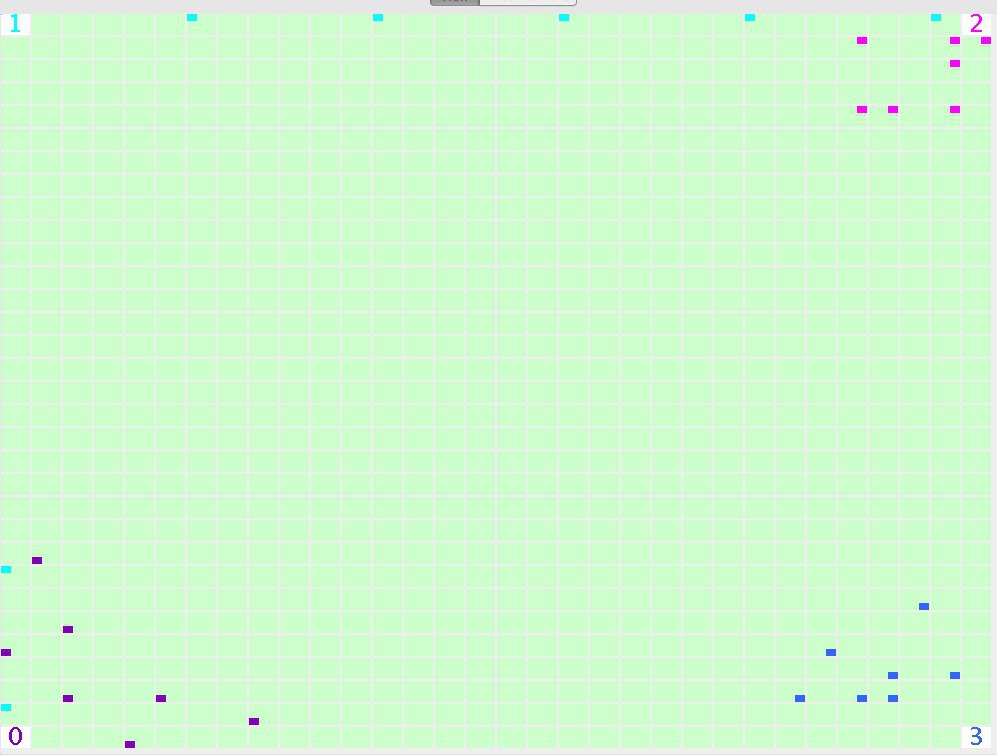
\includegraphics[width=0.8\columnwidth]{initial-position} 
\caption[Initial board of a parallel football game]{An initial positioning of the board where $P=7$}
\label{fig:gallery} 
\end{figure}
\pagebreak

\section{Initial Insights and Observations}

Immediately, our team observed several key features about the game. 

\begin{enumerate}
  \item The game is zero-sum. That is, any ball that is scored by our player is denied to all of our opponents, and vice versa.
  \item Efficiency is not a constraint. Because the game would not progress to the next step until all of our players had calculated their next move, we could take the entire board into account without worrying about the runtime of our solution.
  \item Strategies may work well for certain combinations of $P$ and $K$ and not others. A smart player would change its strategy depending on what value these constants took on.
  \item Certain strategies may work particularly well in the early phase of the game, when all the balls are on the board and there are not clusters, while others may work better in the middle phase (where there are fewer balls and more clusters) or in the end game (when there are only a few balls which every team is competing for).
  \item Efficient strategies (i.e. those which required to fewest moves to kick a ball into the goal) would generally favor kicking over moving, since $K \geq 1$. This naturally leads to a sort of ``bucket brigade'' where players kick balls close to one another in order to ``pass'' them towards the goal.
\end{enumerate}

These insights guided our strategy throughout and allowed us to focus on the most important aspects of the game.

\section{Strategies and Concepts}

\subsection {Movement \& Benefit Function}

In order for a player to decide which cell was the best move for any given board state, we created a benefit function that assigned a score to each cell for every given player. Since we had access to the entire board, we used many factors in this function, including the number of balls in a cell (and surrounding cells), distance from the cell to our goal, distance from the cell to the player, and the number of opponents around the cell. Given the loose efficiency constraints given the problem, we decided that a globally optimal benefit function would be both feasible and desirable. The primary gain from this decision was a team optimized for late gameplay, where our players were able to seek out and steal balls toward the end of the game. The reason was that once we and other teams cleared the balls near our respective goals, balls became scarce. If any team had accumulated balls, even if they were far from our players, they would seek them out and attempt to score with them.

On the other hand, as teams improved, the game time grew shorter and quicker. In such a game, it is possible that a globally optimal zone will change into a depleted zone before a far-away team can reach it. It is likely that our model did not fully capture the constantly changing state of the game board. We addressed this by heavily weighting our own goal in benefit calculations.

\subsection{Benefit Function}
The benefit function was inspired by what we thought a human player would consider while deciding where best to move. We realized that given a point on the board, factors considered while deciding whether or not to move towards that point included not only the Euclidean distance to that point, but also the number of opponents, concentration of balls in the general vicinity of that point, and distance of that point from our home goal. Accounting for the proximity of opponents was particularly important becuase it gave us a measure of how susceptible to change the benefit of a particular cell was: the nearer the opponents, and the higher the number of opponents, the more likely it was for balls in the cell in question to be kicked. This allowed us to take into consideration not just how the board was laid out now, but also gave us a proxy for how each cell might change in the near future.

The following is the benefit function for each cell that was calculated from the perspective of each player on the board so as to allow for the player to move to the cell that offered him the greatest benefit: $$B_{cell} = G_{4 \times 4 cluster} - D_{cell} $$ where $G_{4 \times 4 cluster}$ is the gain offered by that cell and its neighboring cells to the player and $D_{cell}$ is the distance penalty for that cell given the position of the player and the cell. $$G_{4 \times 4 cluster} = $\sum_{cells in 4 \times 4 grid surrounding the cell} \alpha \times numBalls(cell) - \beta \times numOpponents(cell)$ $$ and $$D_{cell} = \gamma \times cellDistanceFromPlayer + \lambda \times numKicksFromCellToOurHomeGoal$$ where $\alpha = 1.2$, $\beta = 0.4$, $\gamma = 1$ and $\lambda = 5$ are weights. These weights were assigned based on the optimal values we found through emperical observations of our performance against other teams over a range of weights.

\subsection{Cell clustering}
On the second iteration of our benefit function, we accounted for ball and opponent clustering by keeping track of the number of balls and opponents surrounding a particular cell. This allowed our players to seek out areas of high benefit, rather than single cells. 

After initial trials with a large radius, we settled on a radius of 4. We observed that larger radii caused the players to move back and forth somewhat inefficiently, and hypothesize that these larger zones changed too quickly for players to capitalize on them.

\subsection{Kicking}
Initially, our players would kick the maximal distance towards the goal. Although this will guarantee that the ball will be as close to the goal as possible, it does not necessarily mean that the number of steps to kick that ball in the goal is minimized when there are teamates around. With this insight, we improved the kicking algorithm with a simple calculation. A player will look at all possible cells it can kick to and minimize the number of steps to kick that ball into the goal for anyone on its team. What this translates to in practice is that a player will now pass the ball as close to a teammate as possible if the teammate is closer to the goal than itself. We observed that after implementing this kicking algorithm, the players naturally form a bucket brigade to minimize the number of steps a player needs to go to for the ball to score.

\subsection{Placement} 
We experimented with several placement strategies. These ranged from clustering near the home goal, near the center, and near opponent goals. We also attempted two hard-coded early-game strategies called \emph{pincer} and \emph{fanned}. Although we eventually opted for a simple clustering around the home goal, we outline some other attempts below.

The \emph{pincer} strategy placed players in lines along the sides adjacent to the home goal, and then swept balls toward the main diagonal, before harvesting them. This strategy aimed to harvest as many easy balls as possible in the very early game, while preventing teams who started in our home goal from "stealing" our balls. After initial testing, it turned out that this strategy quickly fell apart as soon as any opponents interfered with the hard-coded pattern, so we did not retain it in the final implementation. 

The \emph{fanned} strategy placed players on the edges opposite the home goal corner in a $20 \times 20$ grid, and collecting them at "sink points" in increasingly small radii toward the goal. This strategy aimed to fetch 300 of the 400 balls in this grid, assuming thaht 300 was a high enough number to win most matches. The results of this strategy were not great, as we had trouble balancing the tradeoff between systematically sweeping all balls in a zone, and finishing the early-stage sweep quickly enough to switch to a mid-stage strategy. In the end, the configuration was not competitive with our simpler initial placements.

The centered and opponent-goal strategies were somewhat inconclusive in our testing, but generally underperformed the home-goal clustering that we ended up choosing.

The most common opponent strategy was some sort of initial sweep from center-field toward their respective goals. After trying several variants of such strategies, we realized that our players were particularly effective when started from our own goal. Opponents generally swept inwards, carrying some but not all balls from somewhere in the center toward their goal, and then spreading back out to collect what they missed. Starting at the goal, we had a head start at fanning out from the offset and hoped to take advantage of center cells that were left from other team's initial sweeps relatively uncontended.

\section{Implementation}

\subsection{Composability}
Because we realized that certain strategies might work very well in the early phase while others might excel in the late phase, we set about building a player that would \textit{compose} other players by switching between its component players' strategies. We met with a lot of success the second week by composing Group 1's \texttt{GridPlayer} for the first 200 turns and our own mid-game-optimized \texttt{DerickPlayer} for the remainder of the game. This worked about as expected; \texttt{GridPlayer} was far more efficient than \texttt{DerickPlayer} in the early game, but after about 200 turns, the board had grown sparser and our own player was much better at seeking out balls and scoring them. We believed this was the way forward and set about finding a more intelligent way to determine when to switch (factoring in $P$, $K$, and the number of balls left on the board).

However, during the third week of gameplay, the rest of the teams (and our own \texttt{DerickBrigadePlayer}) had become so sophisticated that the early stage of the game completely dominated. Essentially, the winner was determined by how well the early phase played out, and the middle/end phases were nearly nonexistent. Thus we decided to play a pure strategy in the final round, focused on early-game optimization, rather than continuing to compose multiple strategies.

\begin{figure}[h!]
\centering 
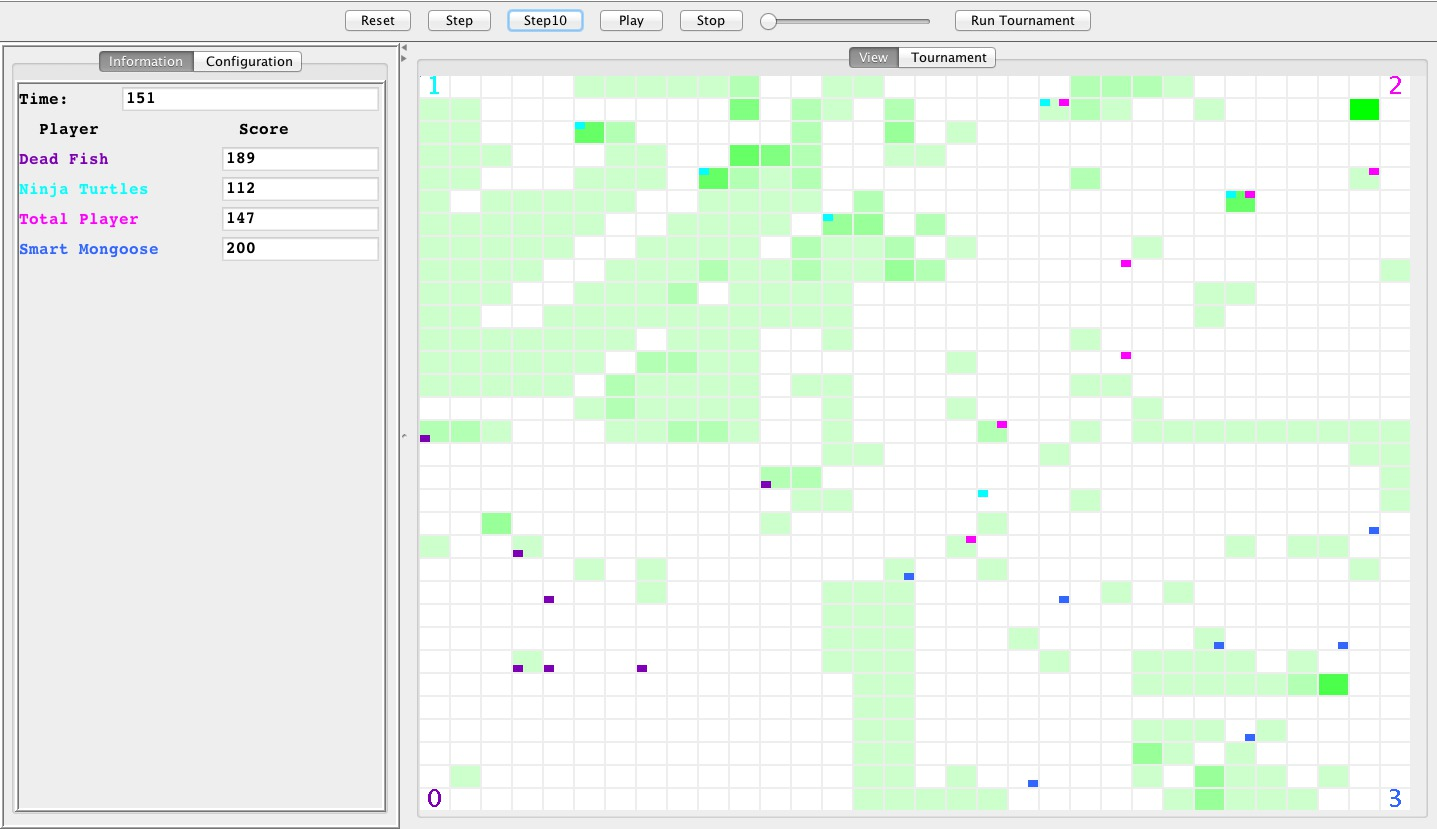
\includegraphics[width=0.8\columnwidth]{after150} 
\caption[State of a parallel football board after 150 turns]{The state of the board after 150 turns with $P=7$, $K=6$. Note how over 60\% of the balls are already scored; this illustrates the great importance of the early game when sophisticated strategies are placed in competition.}
\label{fig:gallery2} 
\end{figure}

\subsection{Placement}
In the early phases, we enumerated the different placement strategies and switched according to values of P and K. Our final implementation was fairly simple, and consisted of a random placement of players near the homegoal, with a bounded parameter on $k$ determining their range.

By starting in a tight cluster bounded by the square from our goal out $MIN(K,10)$ spaces, our players would fan out across the board, while the kicking algorithm led to a trail of $k$-spaced players who formed a bucket brigade. The relatively small square space for player placement was chosen as it balanced the advantages of fanning outward from the goal with scoring an initial $k$-distanced ball for each player.

\subsection{Locking Mechanism}
As we found through our trials, using a benefit function to determine where a player should go runs into problems when players want to go to the same cell. The players will eventually converge and go to the same cells the rest of the game. To prevent this major inefficency, we implemented a locking mechanism where only one player can go after a single cell at a time. However, we found that although this works great through most of the game, when the number of balls is very small, it becomes better for multiple players to go after the same ball to have a higher likelyhood of kicking the ball to the goal. As such, when the number of balls reaches the number of players on the field, we turn off the locking mechanism.

After only locking the cell that the player is going towards, we also lock a radius around that cell. This allows us to create zones such that only one player clearing a zone.Through experimentation, we found that choosing a radius of max(0,3-P/10) works well. With higher number of players, the smaller the zones should become because there is not enough space to create so many zones. Addditionally, it is more likely that opponents will steal balls from a particular zone before a single player can clear that zone out.

\subsection {Auxiliary Board}
The benefit function we used to guide the movement of each player required us to be able to quickly accesss the not only the positions of our own teammates and the balls, but also the positions of our opponents. Moreover, each player needed to know the next postion of every other teammate to ensure smooth kicking and minimal wastage of moves. We encapsulated all this information in an auxiliary board that we refreshed at every time-step. This additional board was a 32 \times 32 2D-array of cells. Each of these cells was an instance of a custom class (Cell) that we created to hold information on the number of opponents, number of teammates now, number of teammates in the next turn and number of balls in the corresponding position on the real board. We found that maintaining this auxiliary board with information specific to our team greatly simplified the code we wrote in other parts of our Player and gave every teammate quick access to decision-critical information. 

\section{Results}
Generally speaking, we had mixed results. Our rank ranged from $1^{st}$ to $7^{th}$ place. Our most common standing was $3^{rd}$ place. We observed that scores followed relative rank, so we chose rank as the proxy for overall performance in the tournaments.

The overall trend in our performance was that we did better than average given low-to-moderate $k$-values (less than 15), and any $p$-values. This makes sense in terms of our initial placement strategy. With very high values of $k$ (at least 30), our players simply started too close to our goal, and did not take advantage of the potential for long-range kicking. Teams starting in the middle were able to clear balls in a single kick, so that even when our players reached the middle sections quickly, there were few balls left. Contrarily, our players remained competitive with smaller $k$. We think that starting players near the goal led to more effective bucket brigading as described in the initial placement section above. Larger values of $p$ did not have a major impact on performance because more players allowed for a more effective covering of the map while maintaining a bucket brigade path back to the goal. It is possible that parameterizing our intitial placement by $p$ as well as $k$ could have improved our scores, but it may have negatively impacted the bucket brigading, and led to similar results.

Two notable configurations are $P,K=45,1$ and $P,K=30,1$. We placed third and first in these categories, respectively. This was a surprise to us, as we had not optimized for single-player configurations at all. We attribute our success here to the globally-optimal strategy we adopted, so that in slower games with long ranges, our player was able to seek out the most beneficial balls and ball clusters across the entire map. This is in contrast with games with higher $p$, where the board layout changed so rapidly that a global-optimized strategy did not provide much benefit. 

Our results are summarized in the following figures. 

\begin{figure}[h]
\centering 
\includegraphics[width=0.8\columnwidth]{ranking-graph} 
\caption[P on the horizontal vs K on the vertical]{P on the horizontal vs K on the vertical axis. Observe the yellow $3^{rd}$ place band for low $k$}
\label{fig:gallery2} 
\end{figure}

\begin{figure}[h]
\centering 
\includegraphics[width=0.8\columnwidth]{ranking-table} 
\caption[Table of rankings per configuration]{Table of rankings per configuration}
\label{fig:gallery2} 
\end{figure}

\section{Contributions}

Just as we adopted many good ideas by other teams (see Acknowledgements section), we contributed two major ideas to the group discussion over the course of the project:

\begin{enumerate}
  \item \textbf{Benefit function - } HI SPRIHA PLZ WRITE THIS
  \item \textbf{Composable Players and Game Phases - } Although we realized early on that the game would likely be characterized by distinct phases in which certain strategies would dominate, it was not until week 2 when other groups really started to pay attention to this idea. This was largely because our performance that week was extremely dominant after we composed \texttt{GridPlayer} in the early game and \texttt{DerickPlayer} for the rest of the round! Other groups began to think about how they could tailor their strategy to perform well in all phases of the game, or at leasthold their own. One group even took this idea to the extreme, creating a \texttt{ReinforcementLearningPlayer} that essentially composed \textit{all} players using a 1NN algorithm!
\end{enumerate}

\section{Future Directions and Limitations}

\subsection{Strengthen Early Game Through Sweeping}
Among teams that placed highly in the tournament, we noticed that their players would tend to start the game by sweeping balls inwards towards their own goal, maximizing their early-game wins before beginning to spread out across the board. Our players, which started close to our own goal, did not exhibit this behavior. Adapting our placement strategy so that they started farther away might be sufficient to achieve this result; however, we could also look into a composability solution in which a sweeping strategy is used for the very first portion of the game before switching to our current players' behavior. This would require significantly tweaking our composability behavior, particularly the point at which the behavior switch occurred, in order to ensure that our players did not continue sweeping for too long before switching to mid-game behavior.

\subsection{Generalized Step Distance}
This idea stems from our attempts to take advantage of global-scope “hotspots,” or high-density ball clusters that are not near the goal. The existing implementation weights balls close to the home goal particularly high, which is good in the early game, but may not be ideal overall. 

\begin{figure}[h]
\centering 
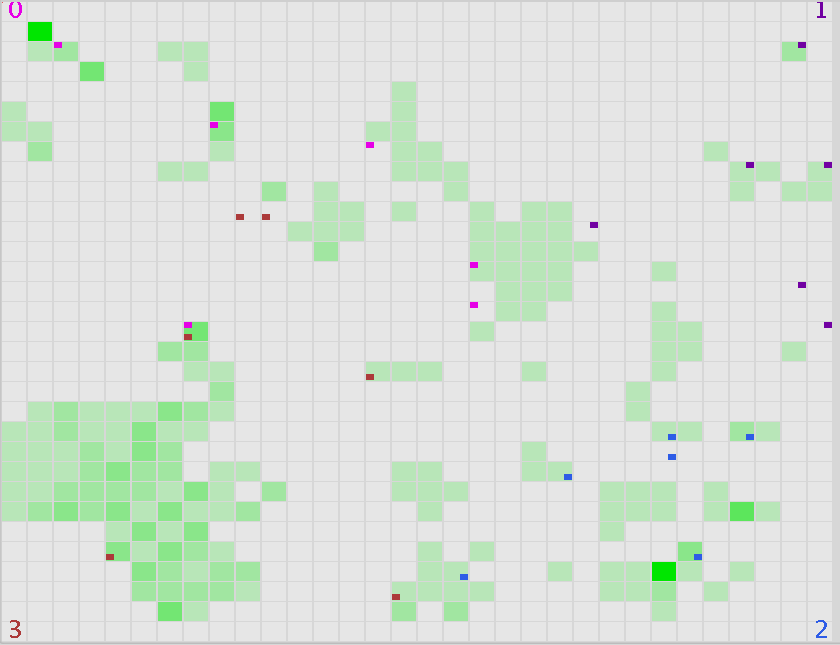
\includegraphics[width=0.8\columnwidth]{hotspot} 
\caption[Example of non-local hotspot]{Example of non-local hotspot after 145 turns with $P=7$, $K=6$. Note how balls are clustered in top bottom-left corner}
\label{fig:gallery2} 
\end{figure}

As we can see in the figure above, certain strategies tend to cluster balls near an opponent goal, where they stay relatively untouched for several cycles. A smarter global-cluster detection would drop the current strategy 

The biggest disadvantage to this approach is that the time it takes to travel to such a cluster may be greater than the the time the cluster exists. Even if the seeking team is able to reach the cluster in time, the balls lost in the transit time may not be worth it.

It would be possible to determine, by factoring in the number of balls left $B_{total}$, the number of balls in close range $B_{nearby}$, and the number of balls expected to remain in the cluster $B_{cluster}$. Such a strategy would decide to go for the cluster if and only if: 
$$B_{total} - B_{nearby} < B_{cluster}$$

One way of implementing this strategy would be to generalize the  \texttt{numberOfStepsToGoal()} benefit function to be \texttt{numberOfStepsToPosition(p)}, where the latter takes in any valid position $p$ as it’s argument, causing the cells around it to get a score boost. Then, upon deciding to pursue a cluster, this position would be updated to the cluster center, until a new position was found.

\subsection{Pathing}
It becomes clear through watching our players that a pathing algorithm could improve our players drastically. We found that our players will often take the same path to their desired locations even though their destinations are distinct. This creates inefficiencies as if there are balls on that path, only one player is needed to clear those balls. In the future, we would look into minimizing the number of cells such that two players would through to reach their destination. 

Another problem with our players with pathing is that they arbitrarily choose a minimum path to its destination. So, if two paths are equally minimal, the player will not choose the path with the most balls, thus missing opportunties to score more points. In the same vein, if two paths are slightly different in the number of steps but the longer path has way more balls, the player will choose the shorter path, causing inefficiencies. To fix this problem, The path the player should take should additionally take into consideration how many balls the player can kick on that path.

\section{Acknowledgments}

Our progress was largely a result of the class discussions and adopted strategies. Through the course of the project, we adopted starting strategies from Groups 1 (Grid Player), as well as experiments in stealing opponent balls with the opening placements. We would like to give special thanks to Groups 2 and 6 for the important heuristics we adopted from them and eventually used in our final implementation. 

Group 2 (The Swarm) was the first group to successfully implement a kind of benefit function with the emergent behavior of a bucket brigade. This function was based on the number of steps from the ball to the goal, and we adopted it as a core feature of our ensemble benefit function.

Group 6 (Bucket Brigade) contributed a smarter kicking function that favored passing to players over kicking as far to the goal as possible. We adopted this idea as a core part of our improved kicking strategy.

\section{Conclusion}

Overall we were happy with the progression of this project and the contributions that our group was able to make to the class, including the benefit function and the composable players. We were also quite pleased with our performance during the second week of the project when our player came out on top!

We hope to take the lessons learned on this project and apply them to later projects in the class. In particular, the idea of optimizing for the early stage of the game (which turned out to be key in parallel football) may prove extremely useful later on as well. Especially in zero-sum games like this one, it can be difficult to stage a come from behind victory when one team starts out with a convincing lead.
\end{document}
